\newlecture
\setcounter{chapter}{9}
\setcounter{section}{0}

\def\coursetopicnumber{II}
\def\textbookchapter{Course Topic II: Multivariable Differentiation}
\def\topic{Functions of Several Variables and Three Dimensional Space} % this is the printed title
\def\shorttopic{Multivariable functions, 3D space} % short topic
\def\textbookname{Active Calculus} % this is the corresponding textbook
\def\shorttextbookname{AC} % this is the short name for the book
\def\textbooksection{9.1B} % corresponding textbook section
\def\textbooksectionurl{https://activecalculus.org/vector/S-9-1-Functions.html} % URL for textbook section
\def\handoutday{} % this is the printed date

\addtocontents{toc}{\bigskip \large \textbookchapter \normalsize \medskip \par} %% for table of contents
%%%%%%%%% DOCUMENT CONTENT STARTS BELOW


\thispagestyle{plain}
\topstuff
\section{(9.1B) \topic{} \booklink{}}
At the start of the course, we covered Section 9.1A (textbook subsections 9.1.1 -- 9.1.3). We'll now cover Section 9.1B (textbook subsections 9.1.4 -- 9.1.6) before getting into Chapter 10. We shift our attention from vector-valued functions to multivariable functions.

\setcounter{subsection}{3}
\subsection{Traces}
Let $f(x,y)$ be a function of two variables defined on some domain in the $xy$-plane. For each point $(x,y)$ in the domain, we have a point $(x,y,f(x,y))$ in $\mathbb{R}^3$. The \emph{graph} of $f$ is the set of all such points $(x,y,f(x,y))$. We often write this as $z=f(x,y)$.

Typically, the graph of a function $f(x,y)$ is a surface in $\mathbb{R}^3$. We'll look at an example from the textbook.

\begin{example}
    Let $f(x,y)=\dfrac{x^2\sin(2y)}{32}$. A sketch of the graph of $f$, for $0\le x\le 220$ and $0\le y\le 1.5$ is given below.

    {\centering 
    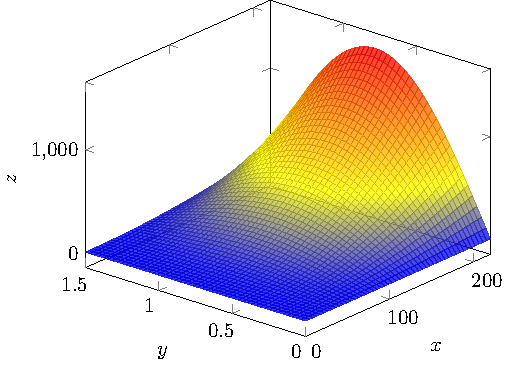
\includegraphics[scale=1]{tikz-pictures/section-9.1-again-pic1-3d-graph-with-traces-1.pdf}\label{img:next-3d-graph}
    \par} 

    \noindent If we intersect this surface with the plane $y=0.6$, we have 
    \[f(x,0.6)=\phantom{\dfrac{x^2\sin(1.2)}{32}}\]
    
    \noindent If we intersect this surface with the plane $x=150$, we have 
    \[f(150,y)=\phantom{\dfrac{150^2\sin(2y)}{32}}\]
    
    The graphs of $z=f(x,0.6)$ and $z=f(150,y)$ are given below.
    
    \pagebreak 
    \mbox{}
    \bigskip 
    
    \begin{center}
        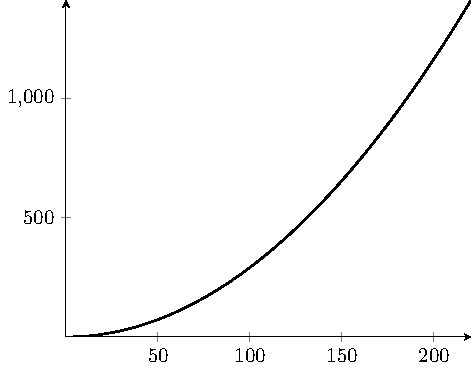
\includegraphics[scale=1]{tikz-pictures/section-9.1-again-pic2-2d-graphs-1.pdf}
        \hfill 
        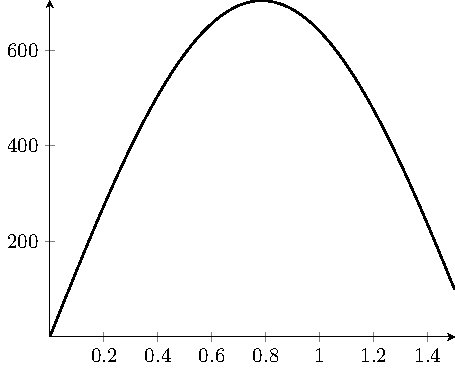
\includegraphics[scale=1]{tikz-pictures/section-9.1-again-pic2-2d-graphs-2.pdf}
    \end{center}
    
    \bigskip 
    
    We can see these graphs on the surface.
    \bigskip 
    
    \begin{center}
        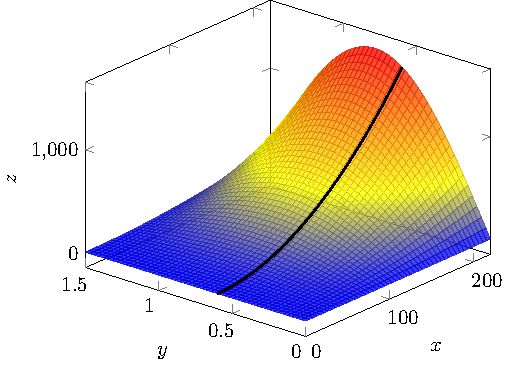
\includegraphics[scale=1]{tikz-pictures/section-9.1-again-pic1-3d-graph-with-traces-2.pdf}
        \hfill
        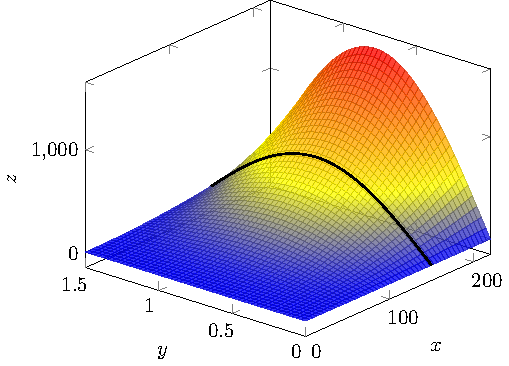
\includegraphics[scale=1]{tikz-pictures/section-9.1-again-pic1-3d-graph-with-traces-3.pdf}\label{img:3d-graph-traces}
    \end{center}
\end{example}

\begin{defn}[Trace]
    An \emph{$x$-trace} of a function $f(x,y)$ is the intersection of the graph of $z=f(x,y)$ with a plane of the form $x=c$, for $c$ constant. In other words, it is the graph of $z=f(c,y)$ in the $yz$-plane.
    
    A \emph{$y$-trace} of a function $f(x,y)$ is the intersection of the graph of $z=f(x,y)$ with a plane of the form $y=c$, for $c$ constant. In other words, it is the graph of $z=f(x,c)$ in the $xz$-plane.
\end{defn}

\pagebreak 

\subsection{Contour maps and level curves}
Here is a side view and an overhead view of some land. The overhead view is called a \emph{topographic map} or \emph{contour map}. Curves on the 3d map are called \emph{contour lines}, and they connect points at the same elevation. On the 2d map, we call them \emph{level curves}
\begin{center}
    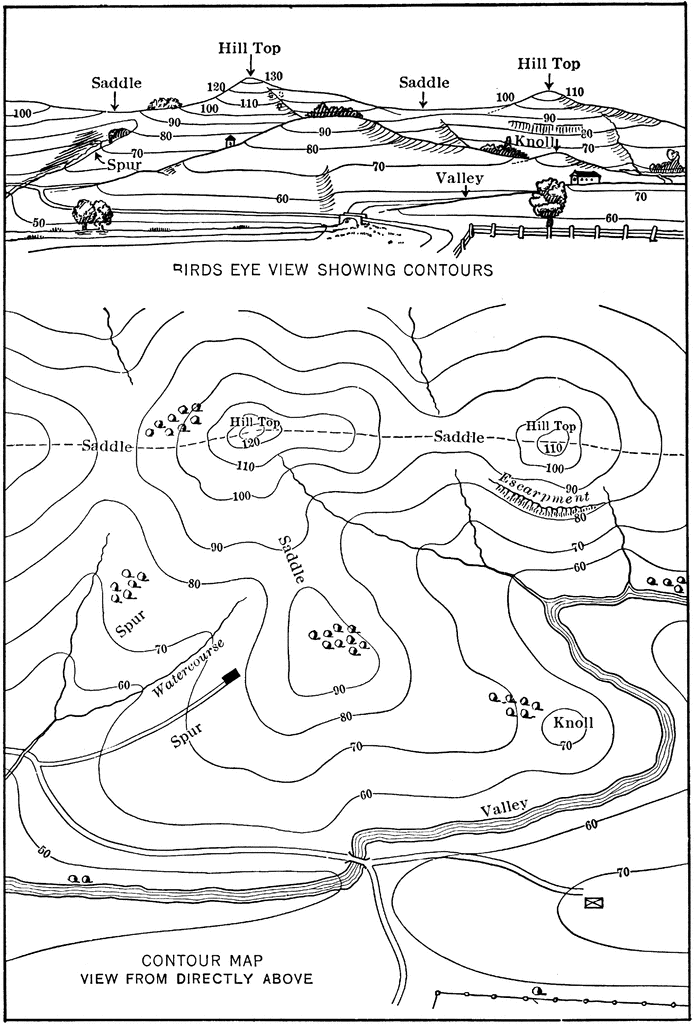
\includegraphics[width=.7\textwidth]{images/contour-map}\label{img:fcit-page-1}
\end{center}

In the context of functions, we can view this map as a portion of $\mathbb{R}^2$. The function $f(x,y)$ that this map represents is the elevation at the point $(x,y)$. In this way, we can visualize a 3D space in a 2D medium.
\vfill\mbox{} 
%\let\thefootnote\relax\footnote{Clipart courtesy FCIT, \href{https://etc.usf.edu/clipart/}{\tt https://etc.usf.edu/clipart/}.}
%\addtocounter{footnote}{-1}\let\thefootnote\svthefootnote
\pagebreak 

Here's another example.
\begin{center}
    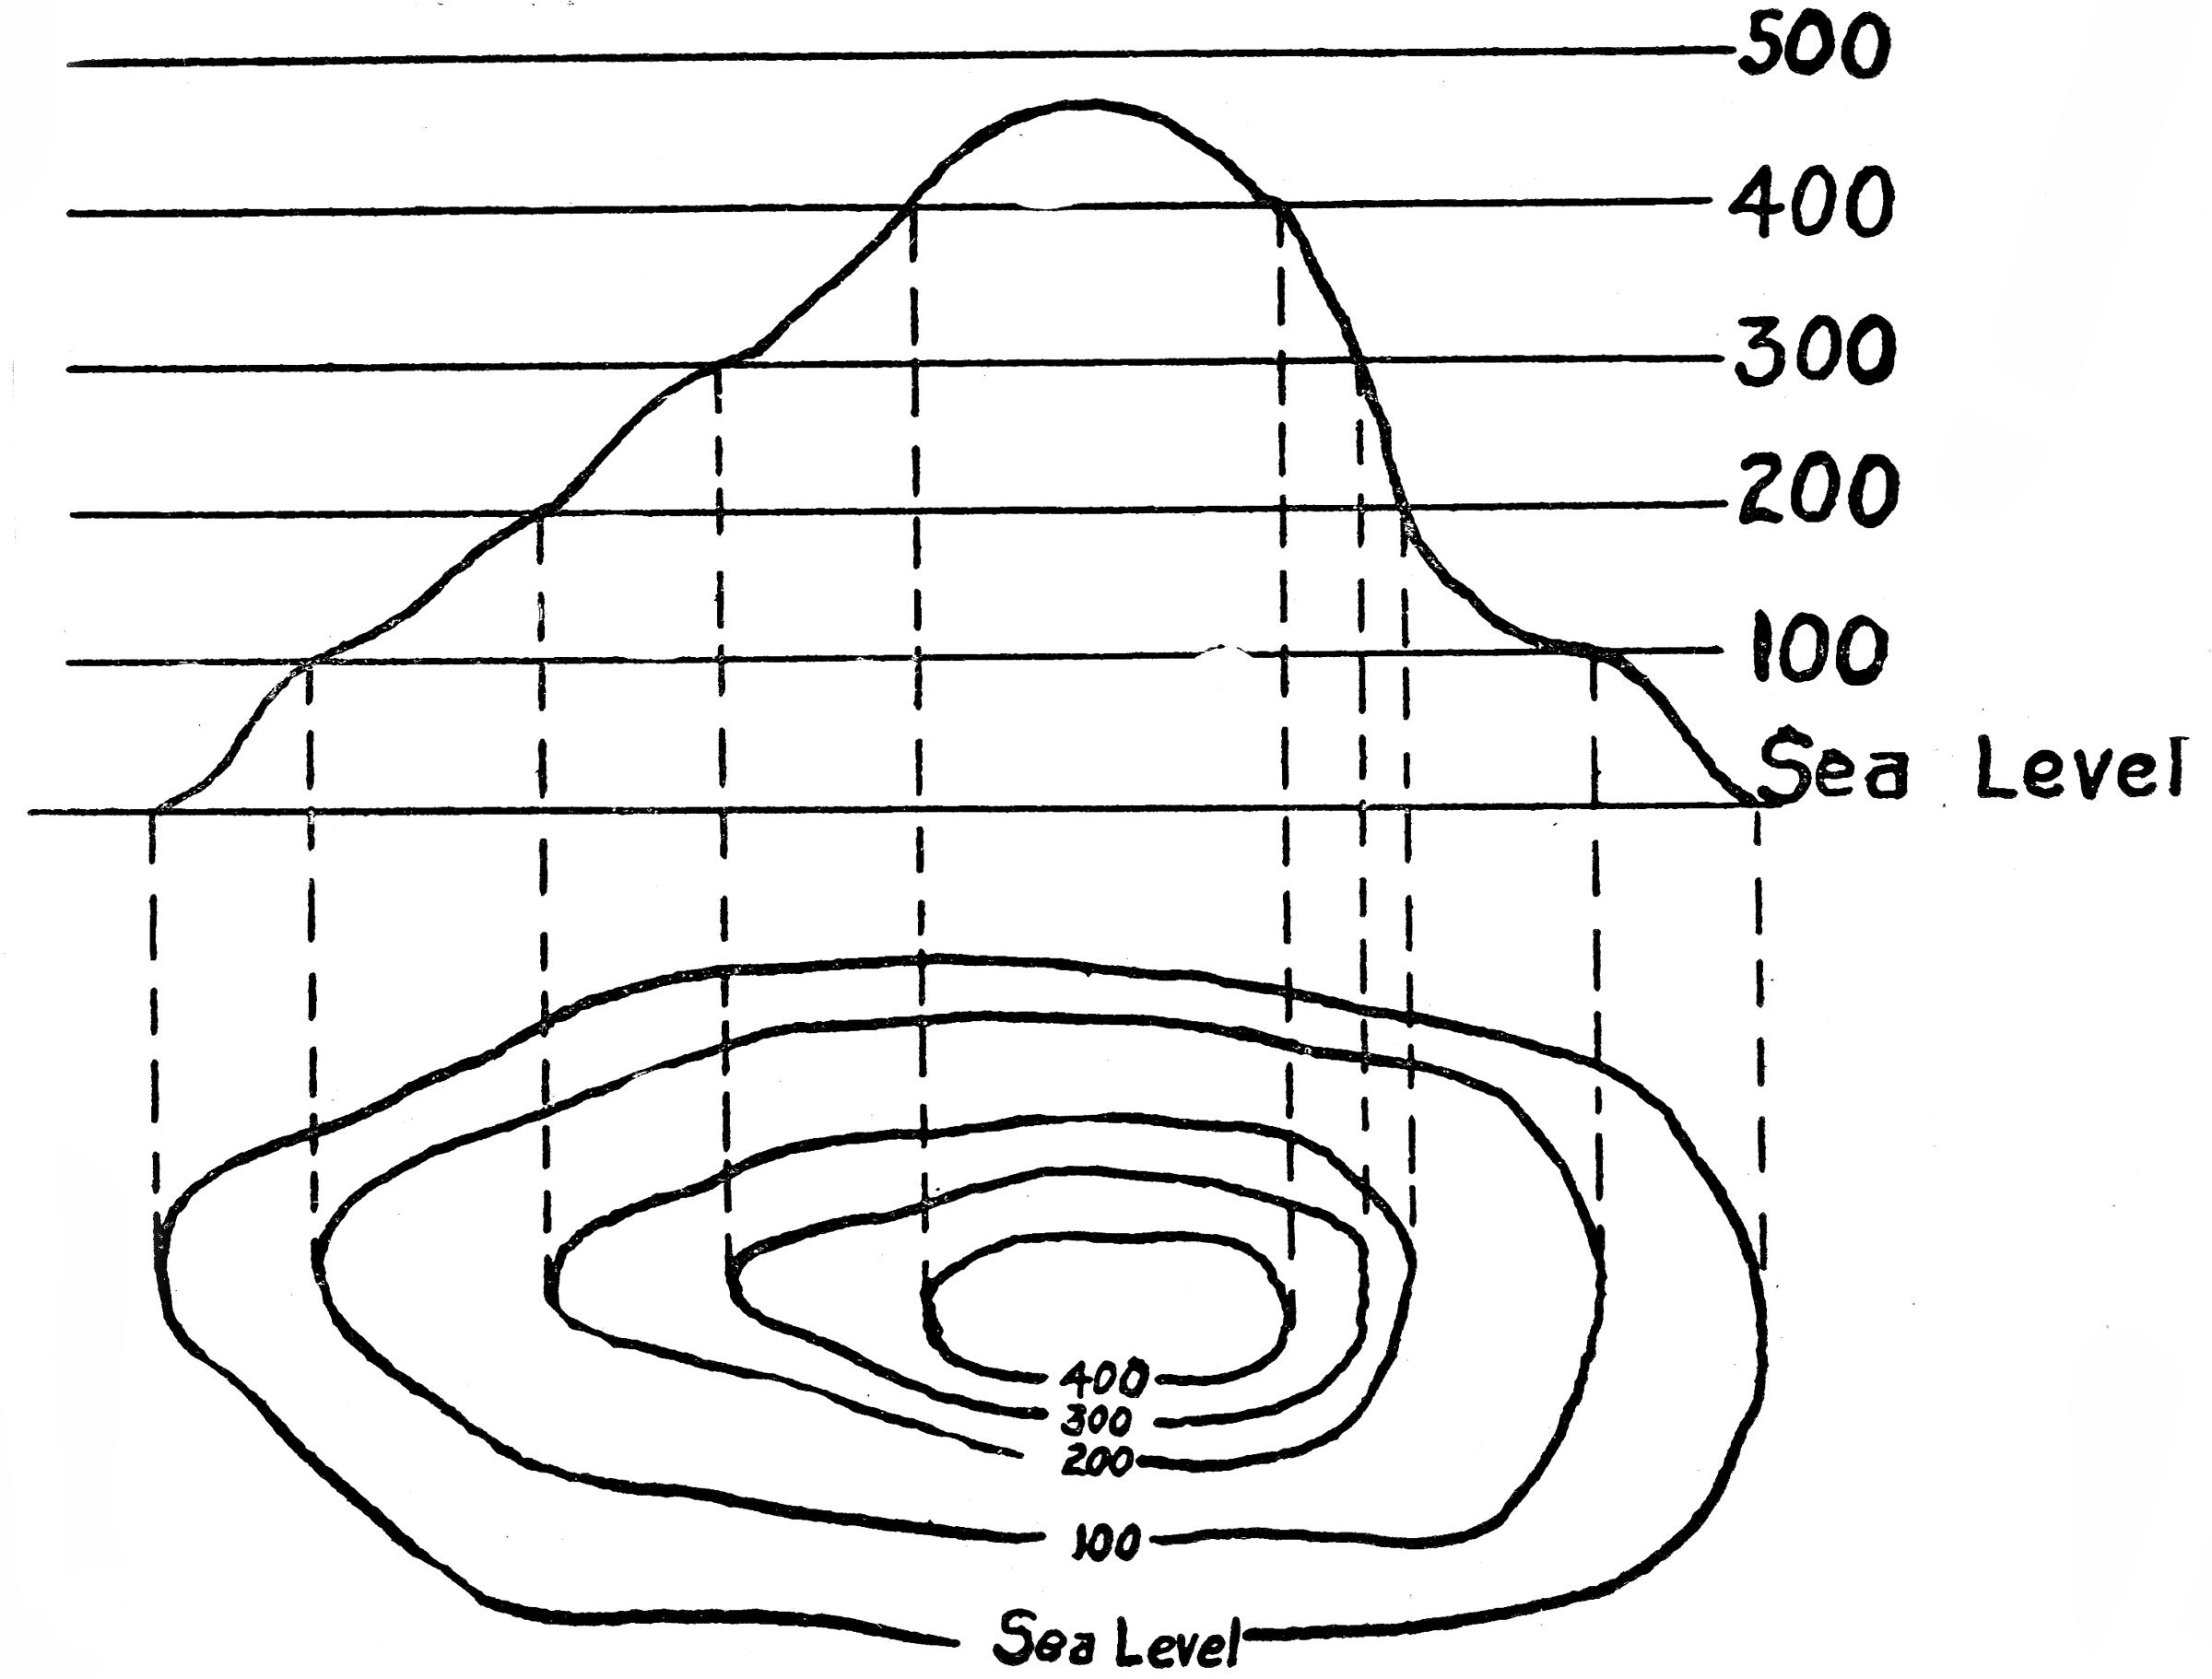
\includegraphics[width=.6\textwidth]{images/topo-map.png}\label{img:fcit-page-2}
\end{center}
\begin{ex}
    Identify major features in the topographic map below.
\end{ex}

\vfill

\begin{center}
    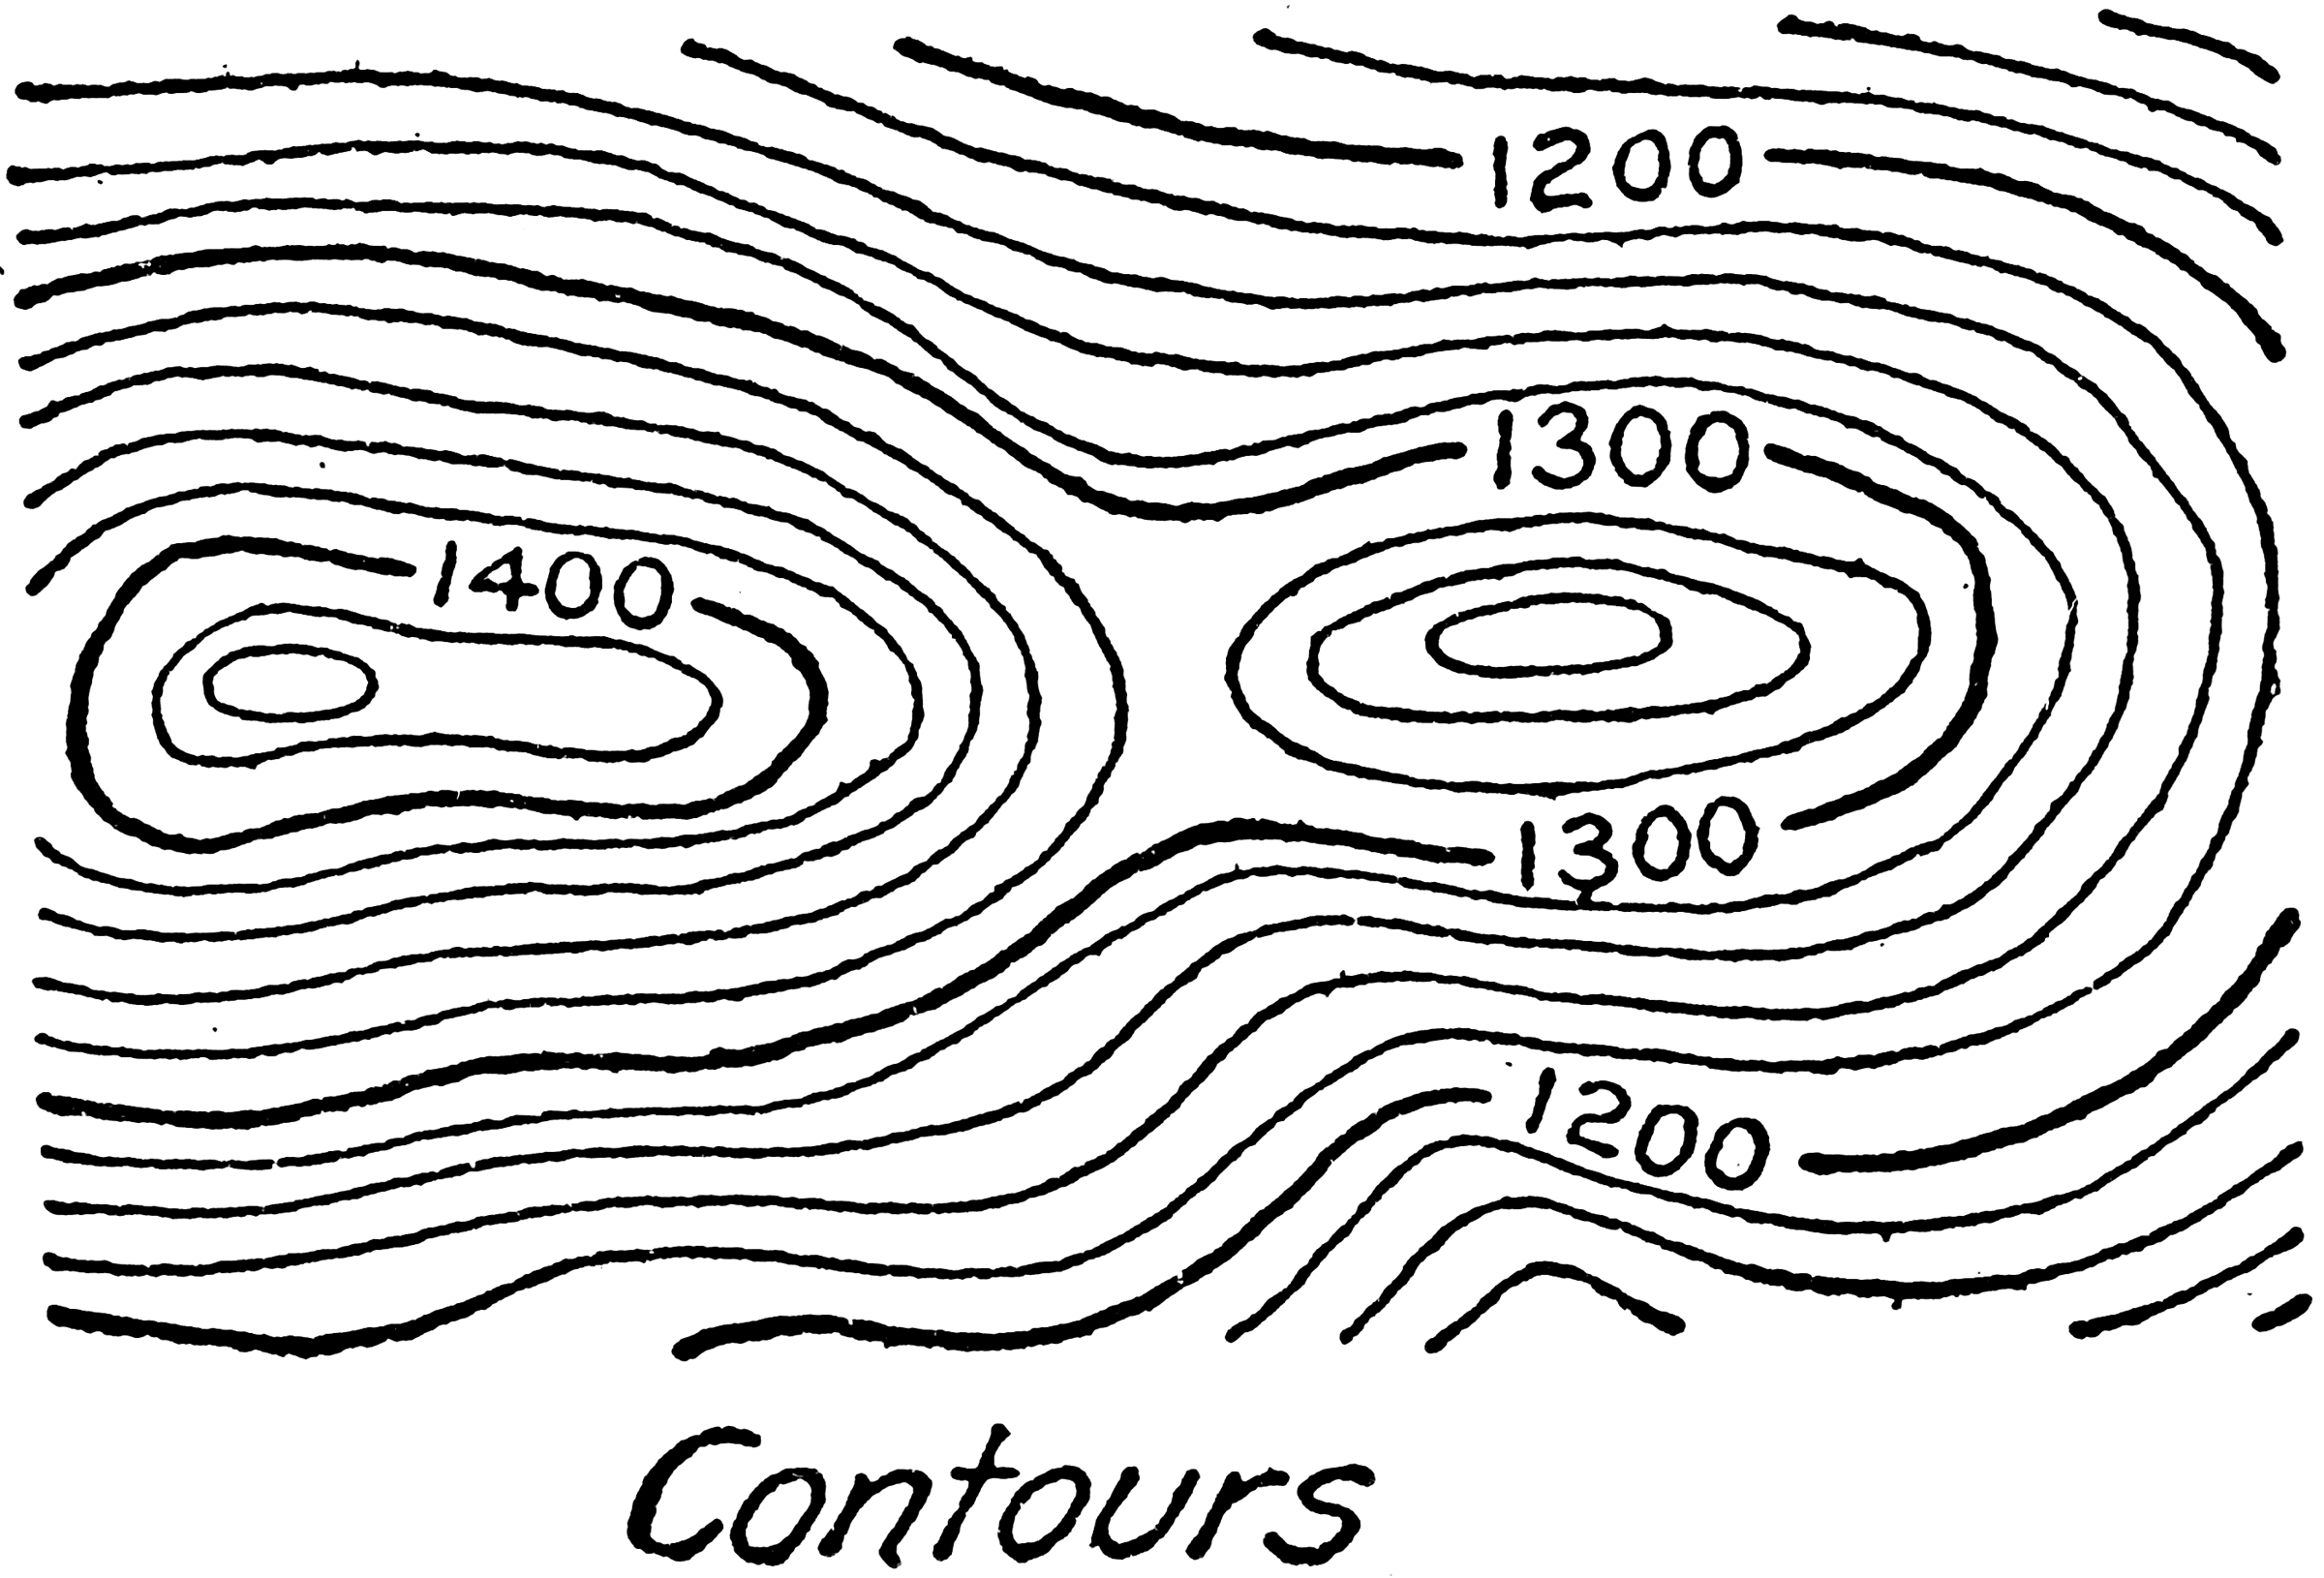
\includegraphics[width=.8\textwidth]{images/topo-map2.png}
\end{center}
\vfill\mbox{} 
%\let\thefootnote\relax\footnote{Clipart courtesy FCIT, \href{https://etc.usf.edu/clipart/}{\tt https://etc.usf.edu/clipart/}.}
%\addtocounter{footnote}{-1}\let\thefootnote\svthefootnote

\pagebreak 

\begin{defn}
    A \emph{level curve} of function $f(x,y)$ is the graph of $f(x,y)=c$ for a constant $c$.
\end{defn}
\begin{ex}\label{ex:elliptic-paraboloid}
    For $f(x,y)=x^2+y^2$, write down the equations of the level curves for $c=0,1,2,\dots,9$. What are these graphs?
\end{ex}
\vfill 

{\centering 
    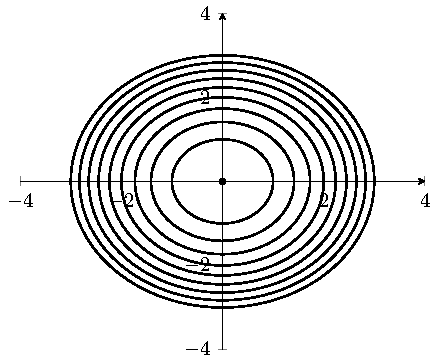
\includegraphics[scale=1]{tikz-pictures/section-9.1-again-pic3-level-curves-elliptic-paraboloid-1.pdf}
\par} 

\begin{center}
    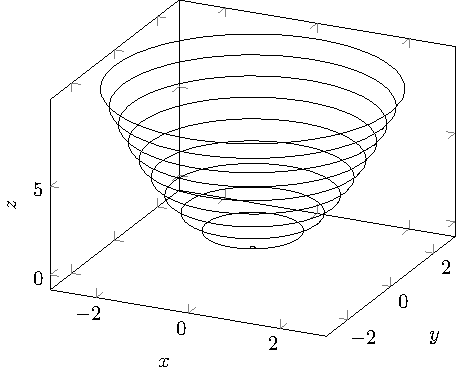
\includegraphics[scale=1]{tikz-pictures/section-9.1-again-pic3-level-curves-elliptic-paraboloid-2.pdf} 
    \hfill 
    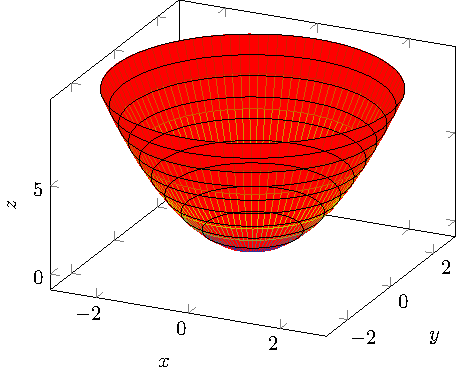
\includegraphics[scale=1]{tikz-pictures/section-9.1-again-pic3-level-curves-elliptic-paraboloid-3.pdf}\label{img:tikz-paraboloid}
\end{center}

\vspace{.5in}

\pagebreak

\begin{ex}\label{ex:cone}
    For $f(x,y)=\sqrt{x^2+y^2}$, write down the equations of the level curves for $c=0,1,2,3,4$. What are these graphs?
\end{ex}

\vfill 

{\centering 
    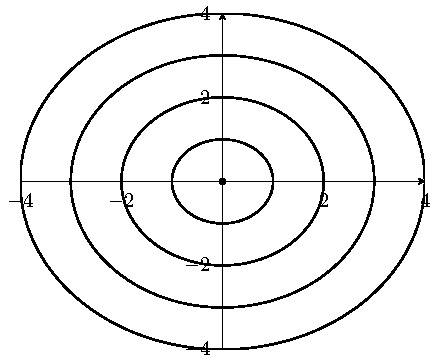
\includegraphics[scale=1]{tikz-pictures/section-9.1-again-pic4-level-curves-cone-1.pdf}
\par} 

\begin{center}
    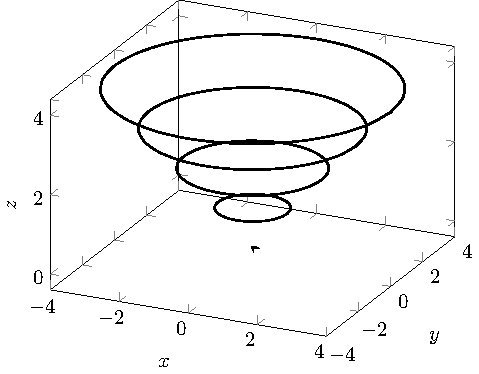
\includegraphics[scale=1]{tikz-pictures/section-9.1-again-pic4-level-curves-cone-2.pdf} 
    \hfill 
    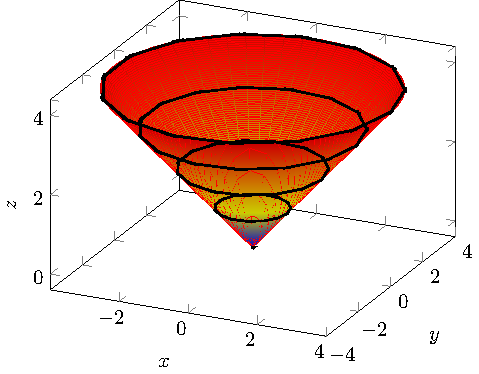
\includegraphics[scale=1]{tikz-pictures/section-9.1-again-pic4-level-curves-cone-3.pdf}\label{img:tikz-cone}
\end{center}

\vspace{.5in}

\pagebreak

\begin{ex}
    For $f(x,y)=-2x-y+6$, write the equations for the level curves for $c=-2,-1,0,1,2$. Sketch the level curves in the $xy$-plane. What does the surface $z=f(x,y)$ look like? Which level curve goes through the point $(x,y)=(4,5)$?
\end{ex}

\vfill\vfill 

\begin{ex}
    Can the level curves of a function cross? Why?    
\end{ex}

\vspace{.5in} 

\begin{ex}\label{ex:shift-bowl}
    We know what the graph of $z=x^2+y^2$ looks like. 
    \begin{enumerate} 
    \item 
    Sketch the graph of $z=(x-1)^2+(y-3)^2$. 
    \item 
    Sketch the graph of $z=4-(x^2+y^2)$.
    \end{enumerate}
\end{ex}

\vfill

\pagebreak

\subsection{A gallery of functions}
In high school geometry, you learned about graphs of low-degree polynomial equations in $x$ and $y$ in $\mathbb{R}^2$.
\begin{itemize} 
    \item Equations of the form $ax+by+c=0$, for constants $a,b,c$, are represented graphically by \emph{lines}. 
    \item Equations of the form $ax^2+bxy+cy^2+dx+ey+f=0$, for constants $a,b,c,d,e,f$, are represented graphically by \emph{conic sections}. These include parabolas, ellipses, and hyperbolas.
\end{itemize}

We now consider low-degree polynomial equations in $x$, $y$, and $z$, and their graphs in $\mathbb{R}^3$. Here are some examples.
\begin{itemize}
    \item The equation $ax+by+cz=d$ graphically is a \emph{plane} with normal vector $\vec{n}=\langle a,b,c\rangle$.
    \item An equation of the form $z=x^2+y^2$ graphically is an \emph{elliptic paraboloid}, or bowl, with vertex at the origin, opening up around the $z$-axis. (Graph given in Exercise \ref{ex:elliptic-paraboloid}.)
    \item An equation of the form $z^2=x^2+y^2$ is an \emph{elliptic cone}, which opens along the positive and negative parts of the $z$-axis. (Top half given in Exercise \ref{ex:cone}.)
    \item An equation of the form $\dfrac{x^2}{a^2}+\dfrac{y^2}{b^2}+\dfrac{z^2}{c^2}=1$ graphically is an \emph{ellipsoid} centered at the origin with radii $a$, $b$, $c$ in the $x-$, $y-$, $z$-directions. When $a=b=c$, we have a sphere.
    \item An equation of the form $z=x^2-y^2$ is a \emph{hyperbolic paraboloid}, or saddle, with flat part at the origin, opening up along the positive and negative parts of the $x$-axis, and opening down along the positive and negative parts of the $y$-axis.
\end{itemize}
As in Exercise \ref{ex:shift-bowl}, we can replace $x,y,z$ with $x-x_0,y-y_0,z-z_0$ to shift a graph. We can also scale variables, swap variables, etc., much in the same way we work with graphs in $\mathbb{R}^2$.

\vfill 

We have seen pictures of planes, elliptic paraboloids, and ellipsoids. Some level curves and a 3D picture of a \emph{hyperbolic paraboloid}, or saddle, which is given by the equation $z=x^2-y^2$, are given below.

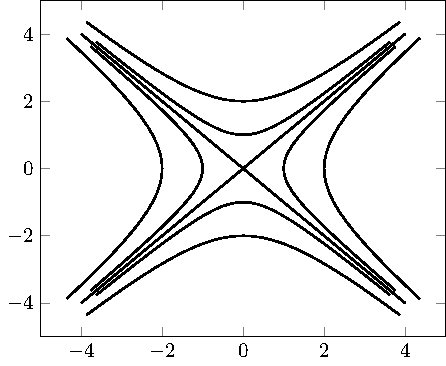
\includegraphics[scale=1]{tikz-pictures/section-9.1-again-pic5-hyperbolic-paraboloid-1.pdf}
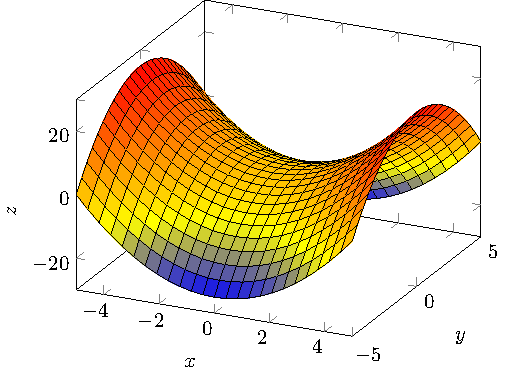
\includegraphics[scale=1]{tikz-pictures/section-9.1-again-pic5-hyperbolic-paraboloid-2.pdf}\label{img:tikz-saddle}

